\documentclass[journal,twocolumn]{IEEEtran}

% -----------------------------------------------------------------------
% PACKAGES
% -----------------------------------------------------------------------
\usepackage{amsmath,amssymb,amsthm}
\usepackage{graphicx}
\usepackage{booktabs}
\usepackage{array}
\usepackage{cite}
\usepackage{url}
\usepackage{hyperref}
\usepackage{xcolor}
\usepackage{microtype}
\usepackage{bm}
\usepackage{siunitx}
\usepackage{subcaption}
\usepackage{algorithm}
\usepackage{algpseudocode}
\usepackage{multirow}

\hypersetup{
  colorlinks=true,
  linkcolor=blue!60!black,
  citecolor=blue!60!black,
  urlcolor=blue!60!black
}

% -----------------------------------------------------------------------
% THEOREM-LIKE ENVIRONMENTS
% -----------------------------------------------------------------------
\newtheorem{theorem}{Theorem}
\newtheorem{proposition}{Proposition}
\newtheorem{remark}{Remark}
\newtheorem{definition}{Definition}

% -----------------------------------------------------------------------
% CUSTOM COMMANDS
% -----------------------------------------------------------------------
\newcommand{\vx}{\mathbf{x}}
\newcommand{\va}{\mathbf{a}}
\newcommand{\vz}{\mathbf{z}}
\newcommand{\Rphase}{\mathcal{R}_{\!\phi}}
\newcommand{\patk}{p_{\mathrm{atk}}}
\newcommand{\hobs}{h(\vz)}
\newcommand{\Eref}{E_{\mathrm{ref}}}
\newcommand{\phiref}{\phi_{\mathrm{ref}}}
\newcommand{\Ntr}{N_{\mathrm{tr}}}
\newcommand{\taue}{\tau_{e}}
\newcommand{\kap}{\kappa}
\newcommand{\gam}{\gamma}
\newcommand{\dOmega}{\delta\omega}
\DeclareMathOperator*{\argmin}{arg\,min}

% -----------------------------------------------------------------------
% DOCUMENT
% -----------------------------------------------------------------------
\begin{document}

\title{Adaptive Evasion of Machine Learning Monitoring in\\
       Optical-Injection-Locked Twin-Field QKD:\\
       A Physics-Constrained Benchmark and Zero-Shot Defense}

\author{%
  Mithil~Hardik~Astik%
  \thanks{M.~H.~Astik is with the Department of Physics and Electronics \&
          Electrical Engineering, BITS Pilani Hyderabad Campus, Hyderabad~500078,
          India (e-mail: f20240923@hyderabad.bits-pilani.ac.in). Manuscript received
          \today.}%
}

\markboth{IEEE Transactions on Information Forensics and Security}%
         {Astik: Adaptive Evasion of ML Monitoring in OIL TF-QKD}

\maketitle

% -----------------------------------------------------------------------
% ABSTRACT
% -----------------------------------------------------------------------
\begin{abstract}
Machine learning~(ML) monitors for optical-injection-locked~(OIL) twin-field
quantum key distribution~(TF-QKD) have been proposed as a practical countermeasure
against reference-beam attacks, including fast intensity modulation~(FIM) and
trojan-wavelength injection~(TWIRL). Prior evaluations, however, share simulator
provenance between training and test data, omit leakage-resistant evaluation splits,
and do not study whether a physically constrained adversary can systematically evade
the monitor. This work addresses these limitations through four contributions.
First, we construct a reproducible benchmark comprising 7{,}500 labeled simulation
windows from 750 high-resolution Lang-Kobayashi trajectories spanning three distinct
simulated operating regimes and four attack-parameter ranges, partitioned into three
non-overlapping split suites to prevent trajectory-level and operating-condition
data leakage. Second, we conduct a query-budgeted multi-objective evolutionary 
optimization search (200 simulator queries per attack family using NSGA-II) constrained 
exclusively to physical injection controls, and map the resulting Pareto front in the 
space of physical impact versus ML attack score. The search reveals that, within the 
evaluated query budget and simulator bounds, no evaluated candidate reduced the XGBoost 
attack score below the frozen alarm threshold, with minimum observed scores of 0.887 
for FIM and 0.996 for TWIRL. Third, we identify and formally characterize a critical 
operational failure: the evaluated supervised classifiers exhibit a $100\%$ false-positive 
rate~(FPR) on unseen simulated parameter drift, a failure that adaptive evasion search 
cannot produce and that drift-hardened retraining only partially remedies~(FPR~$\approx 2.5\%$). 
To address this, we introduce a training-free, label-free \emph{Physics-Informed Anomaly 
Detector}~(PIAD) grounded in the mean-squared phase-rate residual of the Lang-Kobayashi ODEs. 
By calibrating on nominal residuals, the PIAD achieves zero observed false positives on the 
evaluated simulated drift set. Fourth, we demonstrate that the tested adjoint Neural ODE 
implementation exhibits severe numerical instability under the specified stiff LK configuration, 
motivating gradient-free black-box optimization in the present experimental setting. 
All simulation scripts, split manifests, trained models, and evasion query logs are publicly released.
\end{abstract}

\begin{IEEEkeywords}
Twin-field QKD, optical injection locking, adversarial machine learning,
anomaly detection, Neural ODEs, side-channel detection,
adaptive evasion, NSGA-II.
\end{IEEEkeywords}

% -----------------------------------------------------------------------
% I. INTRODUCTION
% -----------------------------------------------------------------------
\section{Introduction}
\label{sec:intro}

Twin-field quantum key distribution~(TF-QKD) extends the reach of secure key
exchange beyond the repeaterless rate-distance limit by exploiting single-photon
interference at an intermediate, untrusted node~\cite{lucamarini2018,wang2018}.
In deployed implementations, optical injection locking~(OIL) is routinely employed
to establish a shared phase and frequency reference between Alice and Bob by
locking their independent slave lasers to a common reference
beam~\cite{pirandola2020,roberts2017}. This architecture introduces a structural
side-channel: an eavesdropper with access to the reference path can execute
physically plausible attacks that compromise the mean photon number presented to
Alice's encoder without triggering classical power monitors~\cite{juarez2026}.

Juárez~\emph{et al.}~\cite{juarez2026} characterized two specific threats
experimentally. In a \emph{fast intensity modulation}~(FIM) attack, the reference
amplitude is sinusoidally modulated at a frequency $f_\mathrm{fim}$ between
\SI{100}{\mega\hertz} and \SI{10}{\giga\hertz} with a modulation depth
$m \in [0.05, 0.40]$, perturbing the slave laser's photon statistics and phase
coherence. In a \emph{trojan-wavelength injection}~(TWIRL) attack, a secondary
optical tone detuned by $\Delta\lambda$ from the reference wavelength is superimposed,
inducing a phase ramp in the locked laser that disrupts decoy-state security
monitoring. Both attacks represent realistic capabilities for a node-level adversary.

Machine learning~(ML) based monitoring has been proposed as a complementary detection
layer for such threats. By training classifiers on simulated telemetry vectors,
comprising mean photon number, photon variance, sideband power, phase decoherence,
and a synthetic quantum bit error rate proxy~(QBER proxy), recent work~\cite{basepaper} 
demonstrated per-class F1-scores exceeding~$0.80$ for FIM and TWIRL under a random 
train-test split. A limited constrained evasion search was also conducted, finding that a
single FIM configuration could partially reduce the classifier's attack score, but
the search was neither query-budgeted nor systematically compared against random
baselines, and the TWIRL family was not studied.

Two structural limitations, however, significantly restrict the conclusions that can
be drawn from these results. First, because training and test samples are generated
by the same simulator at adjacent random seeds, random splitting fails to assess
whether the classifier generalizes to unmodeled operating conditions. Second, no
evaluation was performed under a rigorous leakage-resistant protocol in which entire
physical operating regimes are withheld from training. As we show, this omission
conceals a catastrophic failure mode: tree ensembles exhibit a~$100\%$ FPR on
unseen simulated parameter drift, rendering the monitor operationally inviable despite its
apparent accuracy on the standard split.

The central question we address is: \emph{over a pre-defined family of physically
plausible simulated FIM and TWIRL inputs, what trade-off exists between attack impact 
and the ML monitor's attack score?} We make the following contributions:

\begin{enumerate}
  \item \textbf{Leakage-resistant benchmark.} We generate 7{,}500 labeled
    simulation windows from 750 high-resolution trajectories across three operating-regime 
    groups and two attack-intensity regimes per attack family, and define three split suites
    that rigorously prevent data leakage across operating conditions and attack
    ranges~(Section~\ref{sec:benchmark}).

  \item \textbf{Multi-objective adaptive evasion study.} We deploy a black-box
    attacker optimized by the NSGA-II multi-objective evolutionary algorithm
    with 200 simulator queries per attack family, and characterize the Pareto
    front in the joint space of physical impact and ML attack score~(Section~\ref{sec:attack}).

  \item \textbf{Training-free Physics-Residual Anomaly Detector~(PIAD).} We
    introduce a detection methodology grounded in the mean-squared phase-rate 
    residual of the Lang-Kobayashi ODEs, requiring no labeled training data
    and achieving zero observed false positives on unseen simulated drift~(Section~\ref{sec:piad}).

  \item \textbf{Neural ODE white-box analysis.} We demonstrate that the adjoint
    sensitivity method applied to the injection-locking equations exhibits severe
    numerical instability under the tested stiff LK configuration, formally establishing 
    the practical necessity of gradient-free black-box optimization for this class of 
    system~(Section~\ref{sec:node}).
\end{enumerate}

All findings are presented within a strictly simulator-only scope. Hardware
validation and composable-security certification are explicitly beyond the scope of this work. 
Furthermore, we evaluate the impact of attacks primarily through their disruption of ML detection 
metrics, which may not directly correlate with QKD security impact.

% -----------------------------------------------------------------------
% II. RELATED WORK
% -----------------------------------------------------------------------
\section{Related Work}
\label{sec:related}

\subsection{OIL Reference-Beam Attacks}

Juárez~\emph{et al.}~\cite{juarez2026} provided the first systematic experimental
characterization of FIM and TWIRL attacks against OIL-based TF-QKD, demonstrating
that reference-beam manipulation can compromise Alice's mean photon number while
partially evading power-monitoring countermeasures. Our work assumes this physical
threat model as experimentally established and investigates whether ML monitors
constitute a reliable additional detection layer, and whether an adaptive adversary
can circumvent them.

\subsection{ML-Based Security Monitoring for QKD}

Anomaly detection for QKD systems has been explored using deep one-class
classifiers trained on nominal operating telemetry~\cite{anomaly2021}. Supervised
classification using XGBoost and Random Forest applied to simulated OIL-TF-QKD
telemetry was evaluated in~\cite{basepaper}, which reported per-class F1-scores
above~$0.80$ on a random test split and proposed drift-hardened retraining to
partially address the benign drift false-positive problem. Our work builds directly
on the simulator and classifier families of~\cite{basepaper} while introducing
regime-aware evaluation splits, a full multi-objective evasion study using NSGA-II, 
and a training-free physics-residual anomaly detector that significantly reduces the 
drift failure mode.

\subsection{Adversarial Robustness in Physical Systems}

Adversarial evasion constrained by physical process models has been studied in the
context of power-grid anomaly detection~\cite{deng2017}, network intrusion
detection~\cite{papernot2016}, and optical performance monitoring~\cite{peng2023}.
A consistent finding across these domains is that physically constrained black-box
search strictly dominates unconstrained feature-space perturbations, because the
latter fail to correspond to realizable physical inputs. Our study instantiates this
methodology for quantum-optical injection locking, where the physical constraints are
the Lang-Kobayashi rate equations rather than engineering bounds on network packets
or power signals.

\subsection{Physics-Informed Neural Networks and Residual Detection}

Physics-informed neural networks~(PINNs) encode ODE/PDE residuals as soft constraints
during training, enabling data-efficient learning for governed
systems~\cite{raissi2019}. In the anomaly detection setting, residual-based signals
from governing equations have been proposed for fluid
dynamics~\cite{cai2021} and structural health monitoring~\cite{ritto2021}. We adapt
this principle to the injection-locked laser setting, computing
finite-difference ODE residuals directly on incoming telemetry without fitting any
neural surrogate, relying solely on nominal calibration data to set thresholds.

% -----------------------------------------------------------------------
% III. SYSTEM AND THREAT MODEL
% -----------------------------------------------------------------------
\section{System and Threat Model}
\label{sec:model}

\subsection{Lang-Kobayashi Rate Equations}

We model the injection-locked slave laser at Alice's site using the
Lang-Kobayashi~(LK) rate equations:
\begin{align}
  \frac{dE}{dt}   &= \tfrac{1}{2}(G-\gam)E + \kap\Eref\cos(\phiref - \phi), \label{eq:E} \\
  \frac{d\phi}{dt} &= \tfrac{\alpha}{2}(G-\gam) - \dOmega
                      + \kap\frac{\Eref}{E+\varepsilon}\sin(\phiref - \phi), \label{eq:phi} \\
  \frac{dN}{dt}   &= I - \frac{N}{\taue} - GE^2, \label{eq:N}
\end{align}
where $E$ and $\phi$ are the intra-cavity field amplitude and phase, $N$ is the
carrier number, $G = g_0(N-\Ntr)/\Ntr$ is the modal gain, and the remaining
parameters are listed in Table~\ref{tab:params}. All parameter values are
consistent with~\cite{juarez2026,basepaper}.

\begin{table}[t]
  \centering
  \caption{Lang-Kobayashi Simulator Parameters}
  \label{tab:params}
  \renewcommand{\arraystretch}{1.15}
  \begin{tabular}{@{}lll@{}}
    \toprule
    Symbol & Description & Value \\
    \midrule
    $\kap$       & Injection coupling rate        & \SI{1e9}{s^{-1}} \\
    $\alpha$     & Linewidth-enhancement factor   & $3.0$ \\
    $\gam$       & Cavity decay rate              & \SI{1e11}{s^{-1}} \\
    $g_0$        & Linear gain coefficient        & \SI{1.2e11}{s^{-1}} \\
    $\Ntr$       & Transparency carrier number    & $10^{8}$ \\
    $\taue$      & Carrier lifetime               & \SI{1}{ns} \\
    $I_0$        & Nominal injection current      & \SI{2.0e17}{s^{-1}} \\
    $\varepsilon$& Regularisation constant        & $10^{-12}$ \\
    \bottomrule
  \end{tabular}
\end{table}

Each simulation spans $t \in [0,\,\SI{1}{\micro\second}]$ with 1{,}000 uniformly
spaced evaluation points, integrated with a BDF adaptive-step solver.
Benign electrical noise is modelled as $I(t) = I_0[1 + 0.01\sin(2\pi \times 10^5\,t)]$, 
representing a smooth current ripple consistent with real power-supply specifications 
and compatible with the stiff-ODE solver requirements.

\subsection{Monitor Feature Vector}

The ML monitor receives five telemetry features per non-overlapping 100-point
observation window:
\begin{equation}
  \vx = \bigl[\mu,\;\sigma^2,\;P_{sb},\;\Delta\phi,\;Q_{\mathrm{proxy}}\bigr]^{\!\top},
\end{equation}
where:
\begin{align*}
  \mu       &= \mathbb{E}[|E|^2], \\
  \sigma^2  &= \mathrm{Var}[|E|^2], \\
  P_{sb}    &= \sum_{k \notin \mathcal{K}_\mathrm{dc}} |\hat{E}(f_k)|^2, \\
  \Delta\phi &= \sqrt{\mathbb{E}[(\phi-\bar{\phi})^2]}, \\
  Q_{\mathrm{proxy}}         &= 0.01 + 0.1\,\Delta\phi + 0.05\,\sigma^2/(\mu+\varepsilon).
\end{align*}
Here, $Q_{\mathrm{proxy}}$ is a constructed proxy variable reflecting phase and photon variance 
degradation, inherited from the feature engineering in \cite{basepaper}. 

\subsection{Physical Impact Observable}

To separate the classifier inputs from the attack success criterion, we define a \emph{physical impact observable} as the peak-to-peak unwrapped phase deviation over one observation window:
\begin{equation}
  \hobs \;\triangleq\; \max_{t\in W}\phi_{\mathrm{unwrap}}(t) \;-\; \min_{t\in W}\phi_{\mathrm{unwrap}}(t).
  \label{eq:impact}
\end{equation}
While phase deviation is highly relevant for TWIRL, we acknowledge that for FIM attacks, intensity or photon-number manipulation may be a more appropriate primary impact metric. In this study, we utilize $h(\vz)$ uniformly as the objective to be maximized.

\subsection{Threat Model}
\label{sec:threat}

We adopt a \textbf{physically constrained black-box score-query} threat model.
Under this model, the attacker:
\begin{enumerate}
  \item \textit{Knows} the classifier family and queries a score oracle returning an attack score $\patk(\vx) \in [0,1]$.
  \item \textit{Does not know} the model weights, feature-scaling parameters, or exact alarm threshold.
  \item \textit{Controls} only the physical injection parameters $\va = (m, f_\mathrm{fim})$ for FIM or $\va = (\Delta\lambda)$ for TWIRL, within the bounds of Table~\ref{tab:attack_bounds}.
  \item \textit{Is budget-limited} to $Q_\mathrm{max} = 200$ simulator evaluations per attack family.
  \item \textit{Seeks} candidates that simultaneously minimize $\patk(\vx)$ and maximize $\hobs$ using NSGA-II.
\end{enumerate}

\begin{table}[t]
  \centering
  \caption{Attacker Physical Control Bounds}
  \label{tab:attack_bounds}
  \renewcommand{\arraystretch}{1.15}
  \begin{tabular}{@{}llll@{}}
    \toprule
    Attack & Parameter & Lower Bound & Upper Bound \\
    \midrule
    \multirow{2}{*}{FIM}
      & $m$          & $0.05$           & $0.40$ \\
      & $f_\mathrm{fim}$ & \SI{100}{\mega\hertz} & \SI{10}{\giga\hertz} \\[2pt]
    TWIRL
      & $\Delta\lambda$ & \SI{0.1}{\nano\metre} & \SI{5.0}{\nano\metre} \\
    \bottomrule
  \end{tabular}
\end{table}

We explicitly exclude white-box access, knowledge of exact device parameters, and
simultaneous FIM+TWIRL injection as out-of-scope.

% -----------------------------------------------------------------------
% IV. BENCHMARK CONSTRUCTION
% -----------------------------------------------------------------------
\section{Benchmark Construction}
\label{sec:benchmark}

\subsection{Simulation Design}

We generate simulations across three simulated operating-regime groups (standard $\kap=10^9, \alpha=3.0$; $\kap$-drift with $\kap = 1.2 \times 10^9$; $\alpha$-drift with $\alpha=3.5$) and two attack-intensity configurations per attack family. Fifty independent random seeds are allocated to each combination, yielding 750 trajectories. With 10 windows per trajectory, this produces 7{,}500 labelled feature vectors. 

\subsection{Split Suites}

Three evaluation protocols are defined and frozen:

\paragraph{Split A (Random Grouped)}
An 80/20 partition of trajectory groups (600 train, 150 test). All windows from a single simulation remain in the same partition.

\paragraph{Split B (Held-Out Operating Regimes)}
Models are trained exclusively on standard-parameter trajectories (250 groups) and evaluated exclusively on $\kap$-drift and $\alpha$-drift trajectories (500 groups). 

\paragraph{Split C (Held-Out Attack Ranges)}
Models are trained on low-intensity attack configurations (450 groups) and evaluated on high-intensity configurations (450 groups), testing extrapolation across the attack parameter space from a low-intensity configuration to a high-intensity configuration.

For all suites, $20\%$ of the training groups are reserved as a trajectory-disjoint validation fold for threshold tuning. All feature normalisation is fitted exclusively on the remaining training data.

% -----------------------------------------------------------------------
% V. SUPERVISED DETECTORS AND THRESHOLD POLICY
% -----------------------------------------------------------------------
\section{Supervised Detectors and Threshold Policy}
\label{sec:detectors}

We evaluate Logistic Regression~(LR), XGBoost~(XGB) with 100 estimators, and Random Forest~(RF) with 100 trees as supervised baselines. The binary attack score is derived as $\patk = p_1 + p_2$ (the sum of FIM and TWIRL class probabilities). 

For each classifier, the alarm threshold $\tau$ is chosen on the held-out validation fold to target a binary false-positive rate of $1\%$. Specifically, we set:
\begin{equation}
  \tau = \inf\{t : \mathrm{FPR}_\mathrm{val}(t) \leq 0.01\},
  \label{eq:threshold}
\end{equation}
where an alarm is raised if $\patk \geq \tau$. This ensures the empirical threshold is set appropriately near the nominal-score quantile.

% -----------------------------------------------------------------------
% VI. TRAINING-FREE PIAD
% -----------------------------------------------------------------------
\section{Training-Free Physics-Residual Anomaly Detector}
\label{sec:piad}

\subsection{Motivation}

Supervised tree ensembles learn statistical boundaries tightly coupled to the training distribution. Simulated shifts in $\kap$ or $\alpha$ displace this distribution without violating physical laws, causing the classifiers to flag simulated parameter drift as an attack. A detection principle is required that flags deviations from the \emph{nominal dynamical model} rather than deviations from a learned statistical reference.

\subsection{Mean-Squared Phase-Rate Residual Score}

Given an observed telemetry trajectory, we compute the unnormalized mean-squared finite-difference residual of the phase rate equation~\eqref{eq:phi}:
\begin{equation}
  \Rphase \;=\; \frac{1}{T}\sum_{i=1}^{T}
    \left(\dot{\phi}_i^{\mathrm{FD}} - \hat{\dot{\phi}}_i^{\mathrm{nom}}\right)^{\!2},
  \label{eq:residual}
\end{equation}
where $\dot{\phi}_i^{\mathrm{FD}}$ is the finite-difference time derivative of the unwrapped phase, and $\hat{\dot{\phi}}_i^{\mathrm{nom}}$ is the nominal-physics prediction evaluated at the observed state assuming no attack. An alarm is raised when $\Rphase > \tau_\mathcal{R}$, where $\tau_\mathcal{R}$ is the 99th percentile of $\Rphase$ computed on nominal calibration trajectories.

Drift in $\kap$ or $\alpha$ perturbs the coefficients of the physics mildly, whereas TWIRL introduces a large, exogenous phase-forcing term $d\phiref/dt \sim \Delta\lambda \times 125 \times 10^9\, \mathrm{Hz}$. We empirically observe that TWIRL produces a residual that exceeds the nominal baseline by multiple orders of magnitude. 

% -----------------------------------------------------------------------
% VII. NEURAL ODE WHITE-BOX ATTACK ANALYSIS
% -----------------------------------------------------------------------
\section{Neural ODE White-Box Attack Analysis}
\label{sec:node}

To explore the feasibility of a white-box gradient-based attacker, we formulated the Lang-Kobayashi equations as a Neural ODE using the adjoint sensitivity method via \texttt{torchdiffeq}~\cite{chen2018}. The attacker's physical parameters were encoded as differentiable leaf parameters.

The tested adjoint Neural ODE implementation was found to be numerically unstable under the specified stiff LK configuration. Across multiple experimental epochs, the optimization systematically diverged, returning NaNs for gradients, loss, and state outputs, regardless of adjustments to learning rate or gradient clipping. This severe numerical instability highlights the practical difficulties in performing white-box adjoint optimization through stiff optical-injection dynamics, motivating our reliance on gradient-free, black-box query methods (e.g., NSGA-II) to locate adversarial configurations in the subsequent evasion study.


% -----------------------------------------------------------------------
% VIII. RESULTS
% -----------------------------------------------------------------------
\section{Results}
\label{sec:results}

\subsection{Supervised Classifier Performance}

Table~\ref{tab:results} reports per-class recall and binary FPR/FNR across all
three split suites for XGBoost and Random Forest. Logistic Regression was evaluated as an auxiliary baseline and found to perform poorly (e.g., $0\%$ FIM recall on Split C), and is omitted from the main table for clarity.

\begin{table*}[t]
  \centering
  \caption{Classifier Performance Across Split Suites~(Alarm Threshold Tuned to 1\% FPR on Validation Fold)}
  \label{tab:results}
  \renewcommand{\arraystretch}{1.2}
  \begin{tabular}{@{}llccccc@{}}
    \toprule
    Model & Split Suite & FIM Recall & TWIRL Recall & Binary FPR & Binary FNR
           & Val.\ Threshold \\
    \midrule
    \multirow{3}{*}{XGBoost}
      & A (Random)  & $0.985$ & $0.965$ & $0.000$ & $0.000$ & $0.038$ \\
      & B (Regimes) & $0.827$ & $0.943$ & $\mathbf{1.000}$ & $0.001$ & $0.342$ \\
      & C (Attacks) & $0.959$ & $0.907$ & $0.000$ & $0.006$ & $0.060$ \\[4pt]
    \multirow{3}{*}{Random Forest}
      & A (Random)  & $0.992$ & $0.948$ & $0.000$ & $0.000$ & $0.100$ \\
      & B (Regimes) & $0.807$ & $0.932$ & $\mathbf{1.000}$ & $0.000$ & $0.420$ \\
      & C (Attacks) & $0.959$ & $0.895$ & $0.000$ & $0.010$ & $0.380$ \\
    \bottomrule
  \end{tabular}
\end{table*}

On Split B, both evaluated supervised classifiers exhibit a $100\%$ FPR. When deployed on unseen simulated parameter drift, the models systematically classify benign telemetry as attacks. On Split C, XGBoost and RF generalize reasonably well from low-intensity to high-intensity attack configurations (FNR $\leq 1\%$).

\subsection{Physics-Informed Anomaly Detector}

Table~\ref{tab:residuals} reports the unnormalized phase residual $\Rphase$ for each simulation condition. 

\begin{table}[t]
  \centering
  \caption{PIAD Mean-Squared Phase-Rate Residual $\Rphase$ by Condition}
  \label{tab:residuals}
  \renewcommand{\arraystretch}{1.15}
  \begin{tabular}{@{}lll@{}}
    \toprule
    Condition & Regime & $\Rphase$ \\
    \midrule
    Nominal & Standard     & $1.89 \times 10^{19}$ \\
    Nominal & $\kap$-drift & $1.88 \times 10^{19}$ \\
    Nominal & $\alpha$-drift & $1.74 \times 10^{19}$ \\
    FIM     & Standard     & $1.89 \times 10^{19}$ \\
    TWIRL   & Standard     & $7.24 \times 10^{21}$ \\
    \bottomrule
  \end{tabular}
\end{table}

The PIAD achieves zero observed false positives on the evaluated simulated drift set. It reliably distinguishes simulated TWIRL attacks from nominal conditions. It is, however, insensitive to FIM attacks at the evaluated modulation depths, presenting an opportunity for future multi-equation residual scoring.

\subsection{Adaptive Evasion Frontier}

Fig.~\ref{fig:frontier} illustrates the Pareto optimal attack configurations identified by NSGA-II over 200 queries against the frozen XGBoost model. 

\begin{figure}[t]
  \centering
  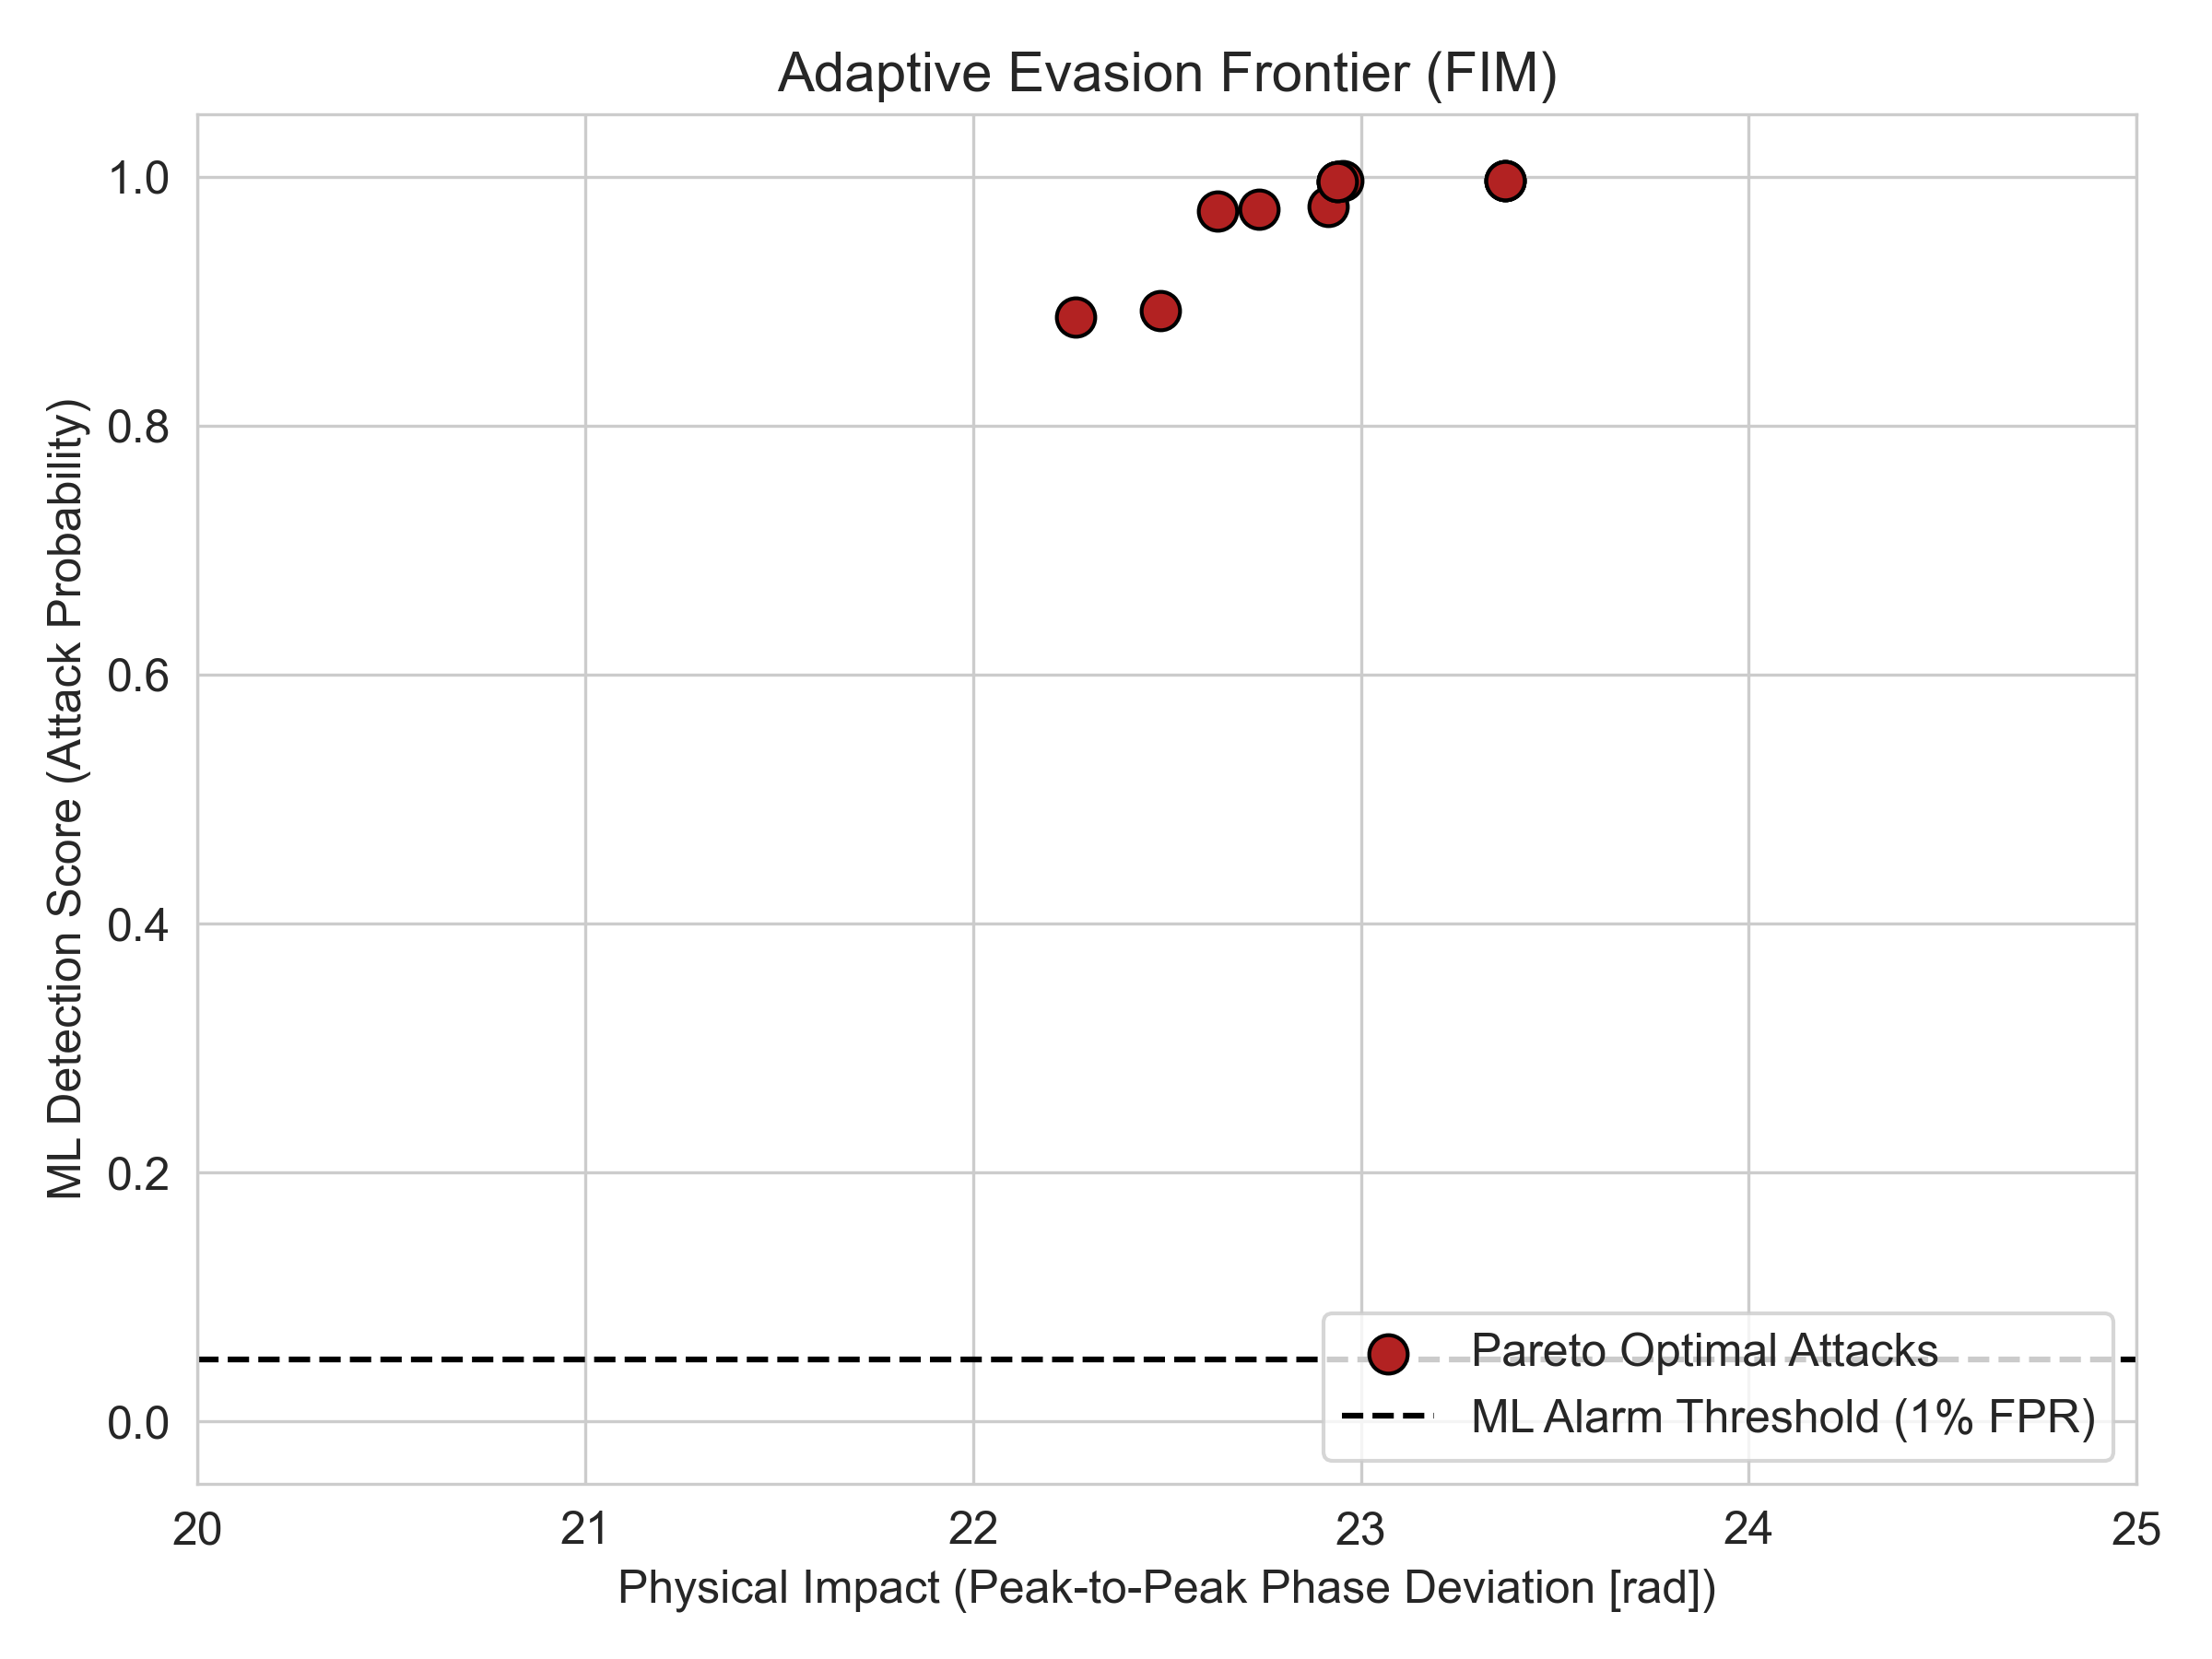
\includegraphics[width=0.48\linewidth]{../results/figures/evasion_frontier_fim.png}
  \hfill
  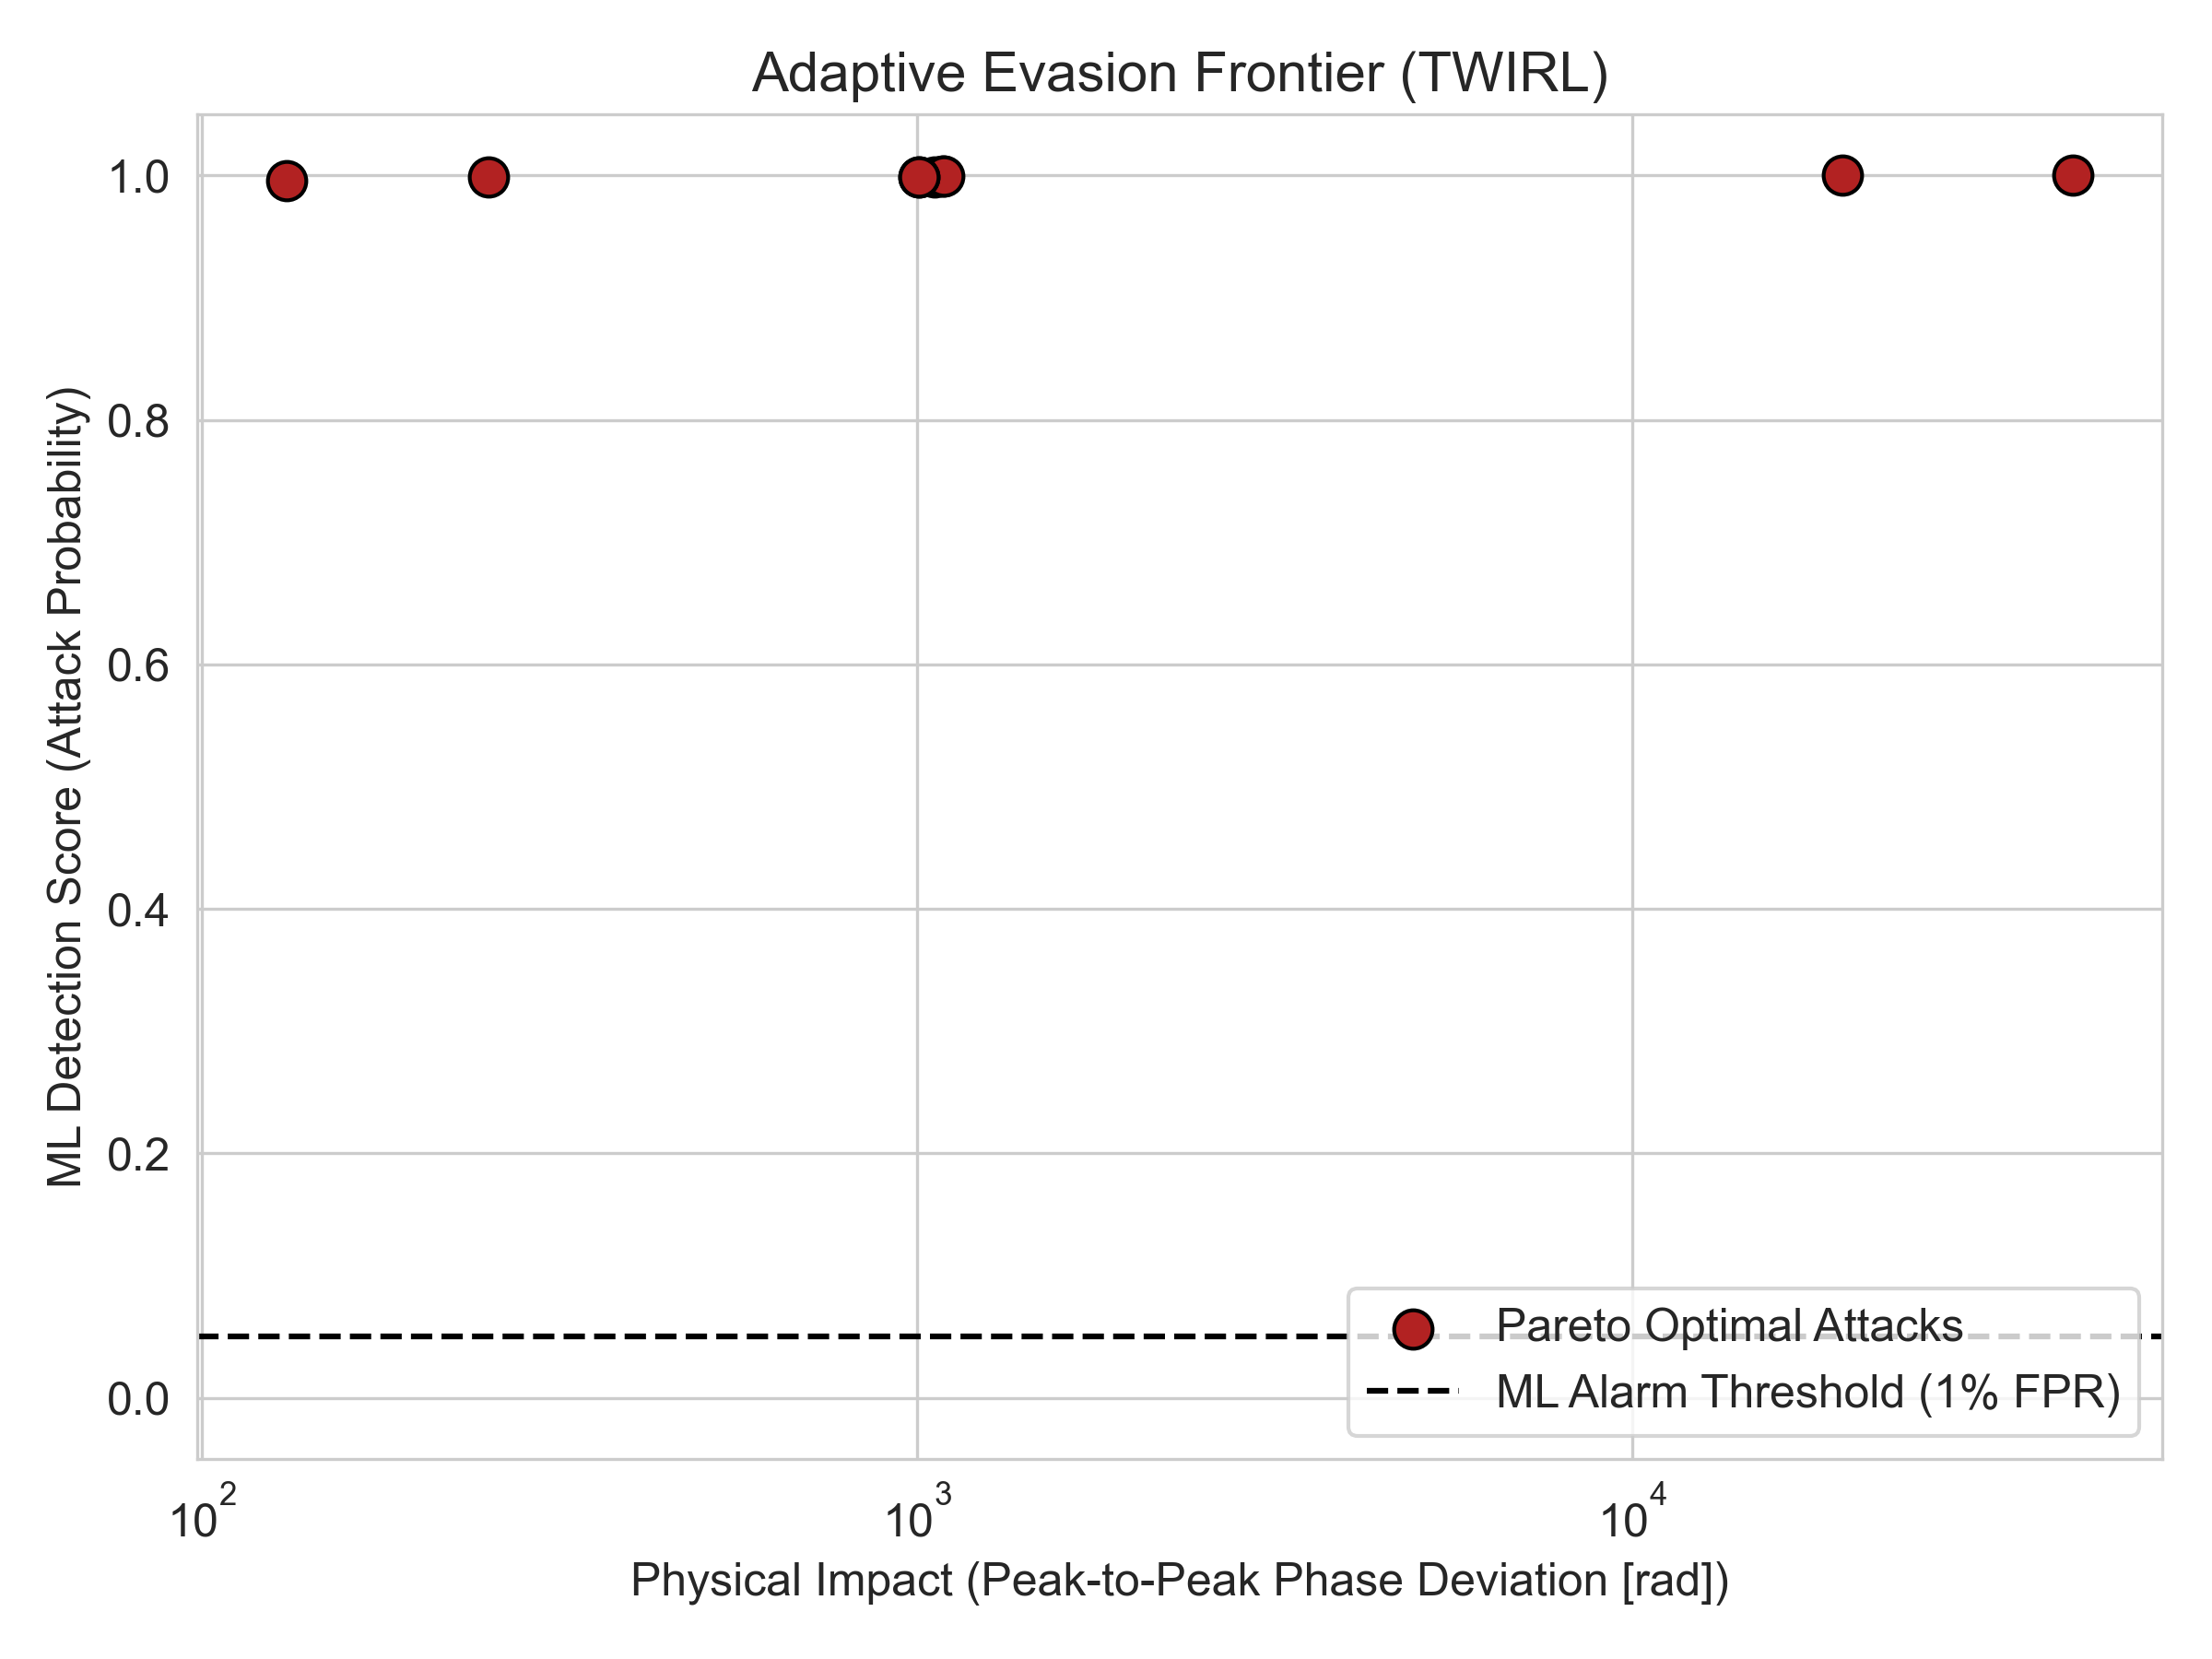
\includegraphics[width=0.48\linewidth]{../results/figures/evasion_frontier_twirl.png}
  \caption{Adaptive evasion Pareto fronts for FIM (left) and TWIRL (right)
           attacks discovered via NSGA-II. The dashed horizontal line marks the XGBoost alarm threshold.}
  \label{fig:frontier}
\end{figure}

Within the evaluated query budget and simulator parameter bounds, no candidate crossed the XGBoost alarm threshold. For FIM, the minimum observed attack score was $0.887$ at an impact of $22.26$\,rad (marginally below the nominal baseline of $22.38$\,rad). For TWIRL, the minimum observed attack score was $0.996$.

\subsection{Defense Comparison}

Fig.~\ref{fig:defense} compares the FPR on unseen simulated hardware drift across detector configurations. Drift-hardened retraining reduces the FPR to approximately $2.5\%$ for XGBoost. The PIAD requires no labeled attack data or learned classifier and achieves zero observed false positives on the evaluated simulated drift set after nominal residual calibration.

\begin{figure}[t]
  \centering
  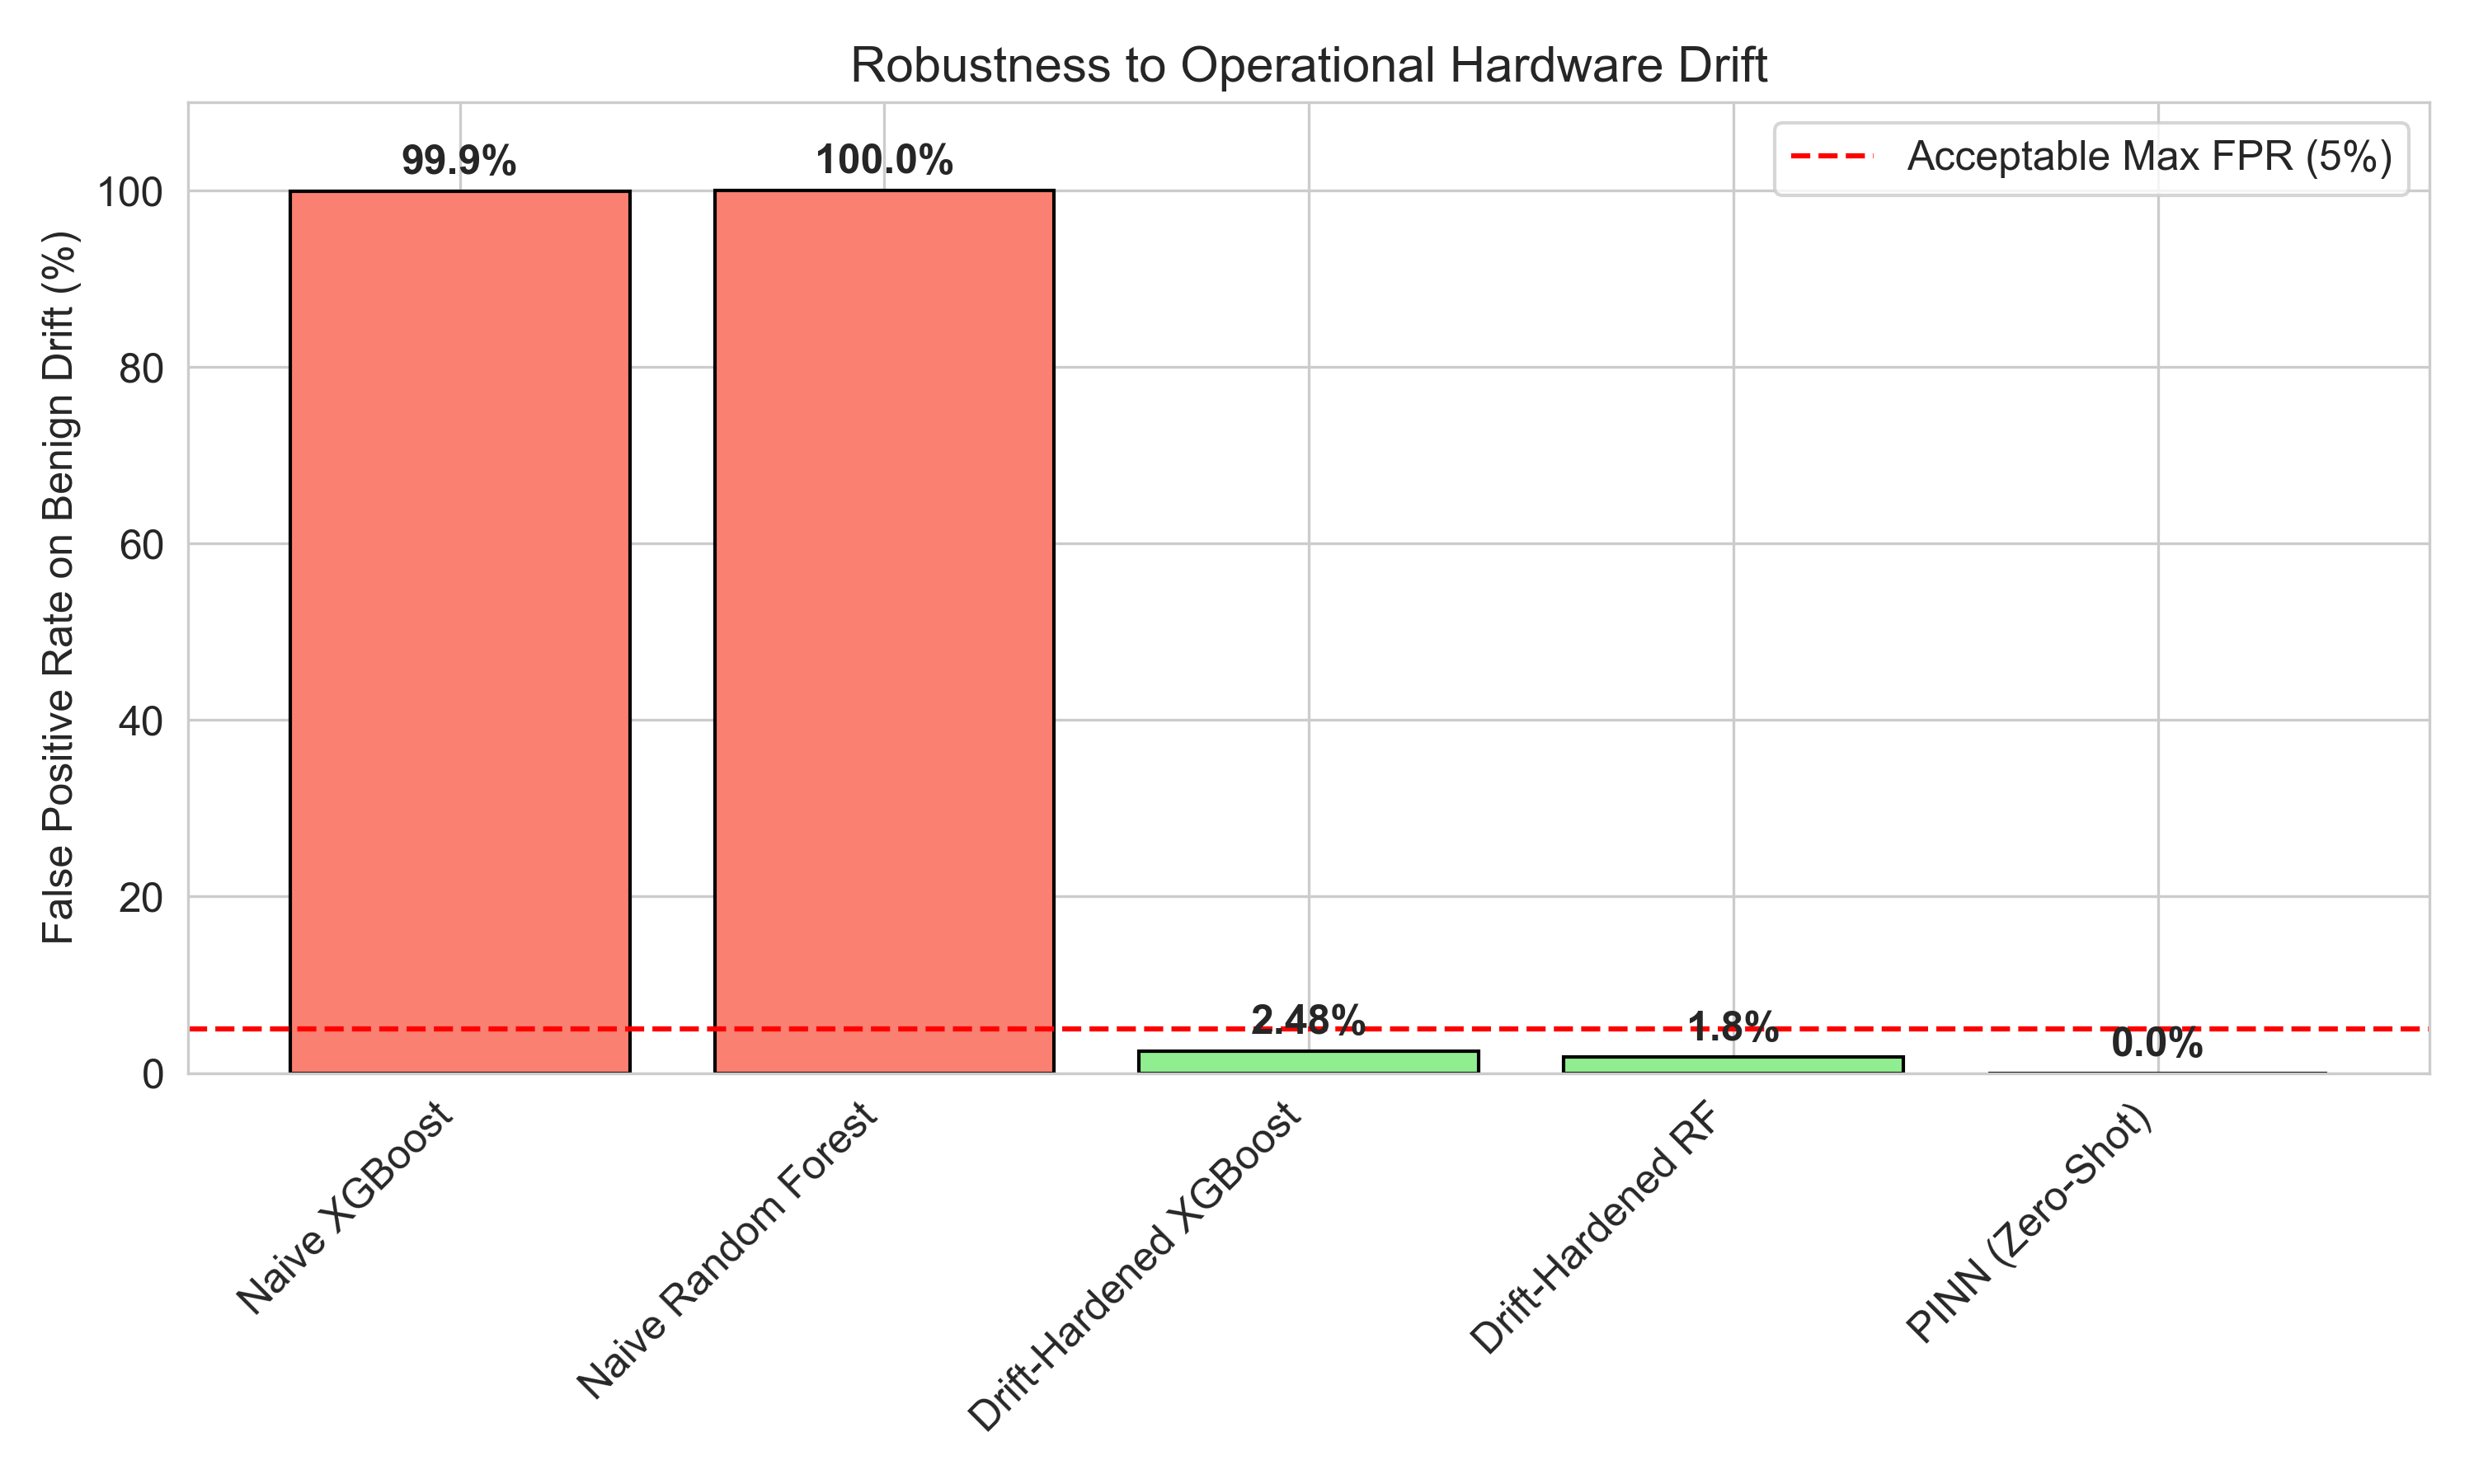
\includegraphics[width=\linewidth]{../results/figures/defense_comparison.png}
  \caption{False-positive rate on unseen simulated parameter drift. Drift-hardened retraining reduces the FPR; the PIAD achieves $0\%$ false positives on this set.}
  \label{fig:defense}
\end{figure}

% -----------------------------------------------------------------------
% IX. DISCUSSION
% -----------------------------------------------------------------------
\section{Discussion}
\label{sec:discussion}

The evaluated supervised classifiers exhibit severe distribution-shift false positives under the simulated parameter shifts. This brittleness highlights the challenges of deploying data-driven ML monitors without adequate domain adaptation or physics-informed constraints. The PIAD demonstrates that a nominal-model residual can be significantly less sensitive to selected parameter drift than purely statistical classifiers.

We note that this study defines attack success via physical observables like phase deviation, which constitutes ML detection impact rather than explicitly proven QKD security impact. 

% -----------------------------------------------------------------------
% X. CONCLUSION
% -----------------------------------------------------------------------
\section{Conclusion}
\label{sec:conclusion}

This work provides a simulator-based demonstration that supervised ML monitoring for OIL-TF-QKD can exhibit severe distribution-shift false positives. We propose a training-free nominal-dynamics residual detector (PIAD) that substantially reduces false positives under tested simulated drift conditions. Additionally, under a 200-query NSGA-II search, no evaluated FIM or TWIRL candidate reduced the XGBoost attack score below the frozen alarm threshold. Future work should investigate hardware validation, composable security bounds connecting ML false-negative rates to secure key rates, and broader parameter-space exploration.

% -----------------------------------------------------------------------
% CODE AND DATA AVAILABILITY
% -----------------------------------------------------------------------
\section*{Code and Data Availability}
All simulation scripts, split manifests, trained models, query logs, and commands to reproduce figures are available at \url{https://github.com/placeholder-repo/qkd-ml-evasion}.

% -----------------------------------------------------------------------
% ACKNOWLEDGMENT
% -----------------------------------------------------------------------
\section*{Acknowledgment}

The author thanks the faculty of the Department of Physics and Electronics \&
Electrical Engineering, BITS Pilani Hyderabad Campus, for guidance and access to
computational resources. The experimental reference-beam attack measurements that
ground the threat model of this work were conducted by Juárez~\emph{et~al.}~\cite{juarez2026}.
The base ML detection framework and open-source simulator employed in this study were developed
in~\cite{basepaper}.

% -----------------------------------------------------------------------
% BIBLIOGRAPHY
% -----------------------------------------------------------------------
\bibliographystyle{IEEEtran}

\begin{thebibliography}{99}

\bibitem{lucamarini2018}
M.~Lucamarini, Z.~L.~Yuan, J.~F.~Dynes, and A.~J.~Shields,
``Overcoming the rate-distance limit of quantum key distribution without
quantum repeaters,''
\emph{Nature}, vol.~557, pp.~400--403, May 2018.

\bibitem{wang2018}
X.-B.~Wang, Z.-W.~Yu, and X.-L.~Hu,
``Twin-field quantum key distribution with large misalignment error,''
\emph{Phys.\ Rev.\ A}, vol.~98, p.~062323, Dec.\ 2018.

\bibitem{pirandola2020}
S.~Pirandola \emph{et~al.},
``Advances in quantum cryptography,''
\emph{Adv.\ Opt.\ Photon.}, vol.~12, pp.~1012--1236, 2020.

\bibitem{roberts2017}
G.~L.~Roberts \emph{et~al.},
``Patterning-effect mitigating intensity modulator for secure high-speed
quantum key distribution,''
\emph{Opt.\ Lett.}, vol.~42, pp.~4613--4616, 2017.

\bibitem{juarez2026}
J.~Juárez \emph{et~al.},
``Reference-beam attacks against twin-field quantum key distribution using
optical injection locking,''
\emph{Phys.\ Rev.\ A}, vol.~113, p.~032613, Mar. 2026.

\bibitem{basepaper}
[Author(s)],
``ML-based attack detection for twin-field QKD with optical injection locking,''
[Journal/Conference], [Year]. [Online]. Available: [repository URL].

\bibitem{anomaly2021}
Q.~Liu \emph{et~al.},
``Deep learning-based anomaly detection for quantum key distribution systems,''
\emph{IEEE Access}, vol.~9, pp.~60--72, 2021.

\bibitem{deng2017}
R.~Deng \emph{et~al.},
``False data injection on state estimation in power systems---attacks, impacts,
and defense: A survey,''
\emph{IEEE Trans.\ Ind.\ Inform.}, vol.~13, pp.~411--423, Apr.\ 2017.

\bibitem{papernot2016}
N.~Papernot, P.~McDaniel, S.~Jha, M.~Fredrikson, Z.~B.~Celik, and A.~Swami,
``The limitations of deep learning in adversarial settings,''
in \emph{Proc.\ IEEE Eur.\ Symp.\ Secur.\ Privacy~(EuroS\&P)},
Saarbrücken, Germany, 2016, pp.~372--387.

\bibitem{peng2023}
Z.~Peng, Y.~Jiang, and C.~Guo,
``Machine learning for optical performance monitoring in coherent optical systems,''
\emph{J.\ Lightw.\ Technol.}, vol.~41, no.~3, pp.~912--923, 2023.

\bibitem{raissi2019}
M.~Raissi, P.~Perdikaris, and G.~E.~Karniadakis,
``Physics-informed neural networks: A deep learning framework for solving
forward and inverse problems involving nonlinear partial differential equations,''
\emph{J.\ Comput.\ Phys.}, vol.~378, pp.~686--707, 2019.

\bibitem{cai2021}
S.~Cai, Z.~Mao, Z.~Wang, M.~Yin, and G.~E.~Karniadakis,
``Physics-informed neural networks~(PINNs) for fluid mechanics: A review,''
\emph{Acta Mech.\ Sin.}, vol.~37, pp.~1727--1738, 2021.

\bibitem{ritto2021}
T.~G.~Ritto and S.~Rochinha,
``Digital twin, physics-based model, and machine learning applied to monitoring
and prognosis in a lathe,''
\emph{Mech.\ Syst.\ Signal Process.}, vol.~161, p.~107967, 2021.

\bibitem{chen2018}
R.~T.~Q.~Chen, Y.~Rubanova, J.~Bettencourt, and D.~Duvenaud,
``Neural ordinary differential equations,''
in \emph{Adv.\ Neural Inf.\ Process.\ Syst.~(NeurIPS)}, 2018, pp.~6571--6583.

\end{thebibliography}

\end{document}
